\chapter{Local Administrator Password Solution}
\section{Einleitung}
Local Administrator Password Solution (LAPS)
%What is it
%Difference to normal (One Admin Password on all, Annoyingly saving password for all, have domain users with local admin permission)

\subsection{Anforderungen}
Um LAPS einsetzten zu können, wir ein Active Directory benötigt.



\section{Installation}
Die Installation ist in drei Schritte unterteilt.
Als erstes wird LAPS per Group Policy auf allen Windows Geräten installiert.
Danach wird das Active Directory für LAPS vorbereitet.
Das Active Directory braucht noch zwei zusätzliche Attribute auf den Computer Objekten.
\begin{itemize}
    \item \textbf{ms-Mcs-AdmPwd}: Speichert das Administrator Passwort in Plain-Text.
    \item \textbf{ms-Mcs-AdmPwdExpirationTime}: Speichert den Zeitpunkt für den Passwortwechsel.
\end{itemize}

Zum Schluss wird LAPS per Group Policy aktiviert.


\subsection{Softwareverteilung}
LAPS kann auf der \href{https://www.microsoft.com/download/details.aspx?id=46899}{Webseite von Microsoft}\footnote{Link: https://www.microsoft.com/download/details.aspx?id=46899} heruntergeladen werden.
Die .msi Datei muss in einem freigegebenen Netzlaufwerk auf dem Domain Controller platziert werden, auf welches alle Windows Geräte Zugriff haben.
Zum Beispiel: \textbf{C:\textbackslash Windows\textbackslash SYSVOL\textbackslash sysvol\textbackslash <domain>\textbackslash}.
Dieses Verzeichniss ist Standardmässig auf Domain Controllern freigegeben.\\

Im Group Policy Management muss eine neue Group Policy erstellt werden, welche mit der OU verknüpft ist, die alle Windows Geräte enthält.
\begin{figure}[H]
    \centering
    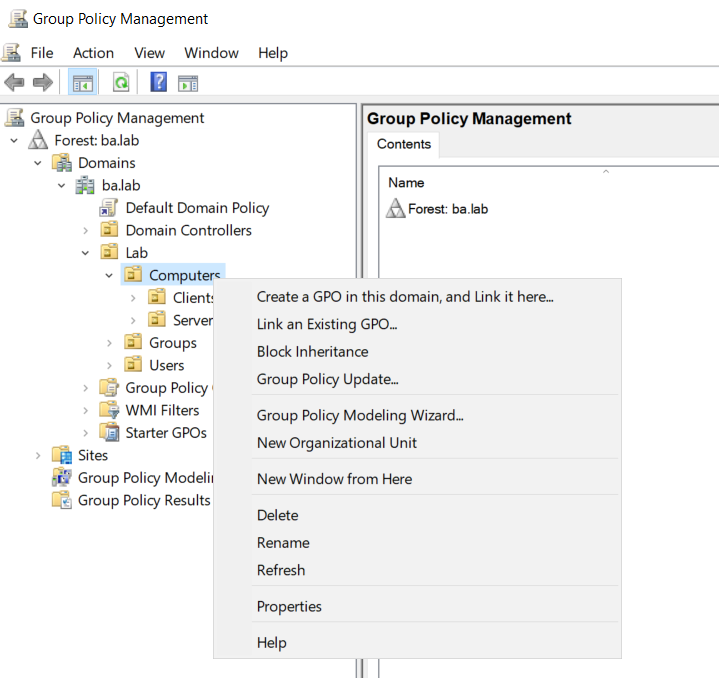
\includegraphics[width=0.7\linewidth]{../img/LAPS/GPO-Create-New.png}
    \caption{Neue GPO für LAPS Deployment}
\end{figure}

Mit \textbf{Rechtsklick $\rightarrow$ Edit} kann die neue Group Policy bearbeitet werden.
Unter \textbf{Computer Configuration $\rightarrow$ Policies $\rightarrow$ Software Settings $\rightarrow$ Software installation} kann mit \textbf{Rechtsklick $\rightarrow$ New $\rightarrow$ Package\dots} eine Datei ausgewählt werden, welche installiert werden soll.
Hier muss man die zuvor im freigegebenen Netzlaufwerk abgelegte Installationsdatei auswählen.
\begin{figure}[H]
    \centering
    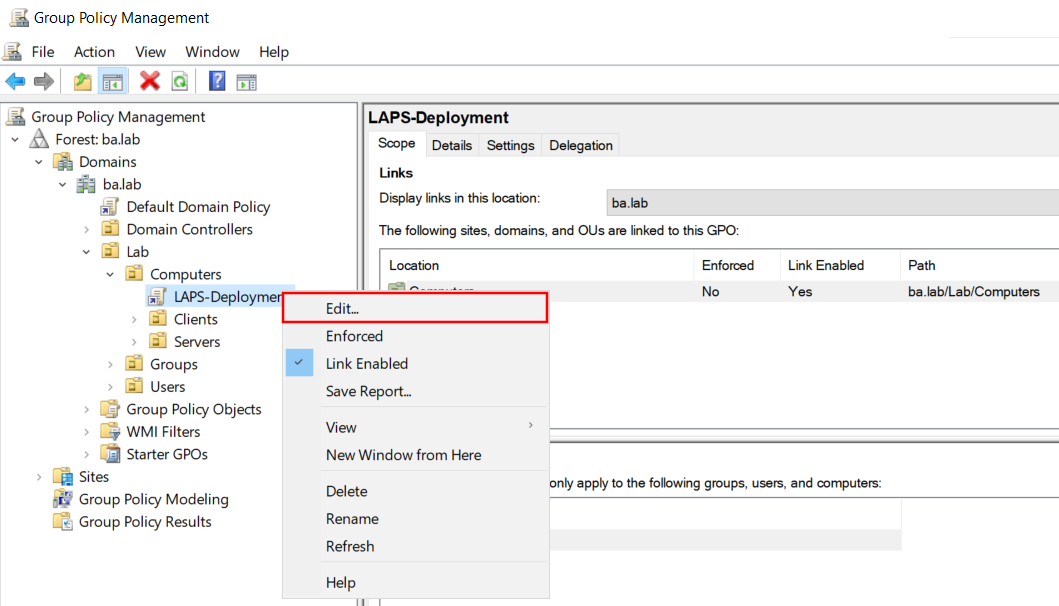
\includegraphics[width=0.7\linewidth]{../img/LAPS/GPO-Edit-Deployment.png}
    \caption{GPO für LAPS Deployment bearbeiten}
\end{figure}

\begin{figure}[H]
    \centering
    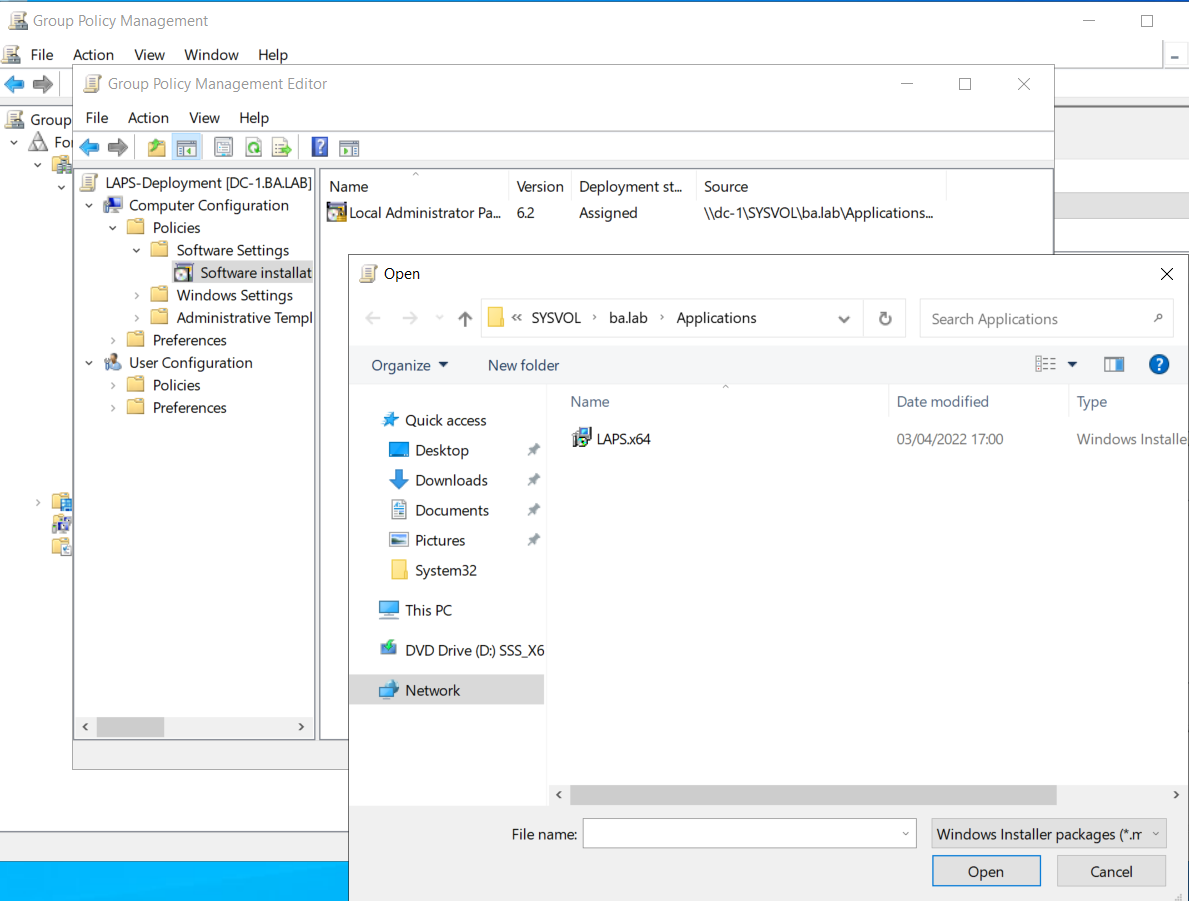
\includegraphics[width=0.7\linewidth]{../img/LAPS/GPO-Edit-Deployment-2.png}
    \caption{LAPS Installationsdatei auswählen}
\end{figure}
Die Group Policy kann nun geschlossen werden.
LAPS wird beim Einloggen auf den jeweiligen Geräten installiert.


\subsection{LAPS GUI für Admins}
Über die GPO wird auf den Computern LAPS ohne GUI installiert.
Mit dem GUI kann man das Passwort von beliebigen Windows Geräten abfragen.\\

In der Programmliste in den Systemeinstellungen auf LAPS klicken und im Balken auf \textbf{Change} klicken.
\begin{figure}[H]
    \centering
    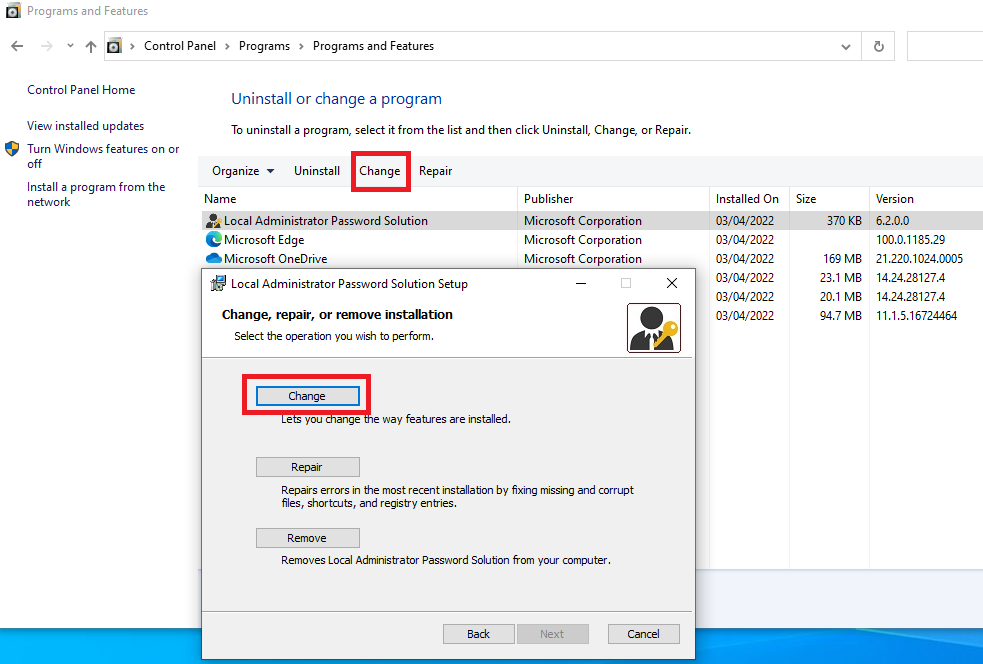
\includegraphics[width=0.7\linewidth]{../img/LAPS/laps-ui-install.png}
    \caption{LAPS GUI Installieren 1}
\end{figure}

Das \textbf{Management Tools} Feature auswählen und dem Installationsprozess folgen.
\begin{figure}[H]
    \centering
    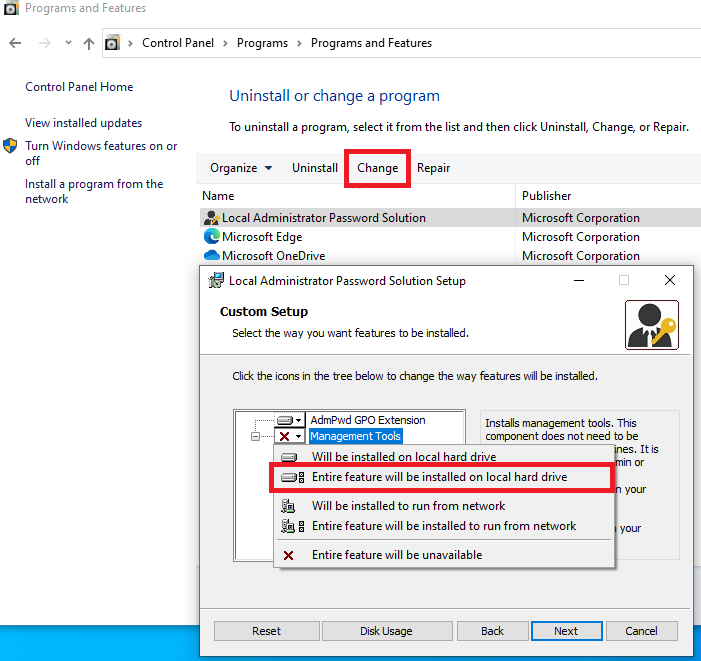
\includegraphics[width=0.7\linewidth]{../img/LAPS/laps-ui-install-2.png}
    \caption{LAPS GUI Installieren 2}
\end{figure}


\subsection{Active Directory vorbereiten}
Die zusätzlichen Extension Attributes können per Powershell hinzugefügt werden.
Der Auszuführende Benutzer muss dafür ``Schema Admin'' sein.\\

Powershell mit dem Schema Admin Benutzer starten.
\begin{lstlisting}
Import-module AdmPwd.PS
Update-AdmPwdADSchema

#Resultat:
Operation            DistinguishedName                                              Status
---------            -----------------                                              ------
AddSchemaAttribute   cn=ms-Mcs-AdmPwdExpirationTime,CN=Schema,CN=Configuration,DC=b Success
AddSchemaAttribute   cn=ms-Mcs-AdmPwd,CN=Schema,CN=Configuration,DC=ba,DC=lab       Success
ModifySchemaClass    cn=computer,CN=Schema,CN=Configuration,DC=ba,DC=lab            Success

Set-AdmPwdComputerSelfPermission -OrgUnit "<Name der OU>"
#Resultat:
Name                 DistinguishedName                                              Status
----                 -----------------                                              ------
Clients              OU=Clients,OU=Computers,OU=Lab,DC=ba,DC=lab                    Delegated
\end{lstlisting}

Nun muss noch eine Active Directory Gruppe erstellt werden.
Dieser kann man alle Benutzer hinzufügen, welche Zugriff auf die Passwörter bekommen sollen.

\begin{figure}[H]
    \centering
    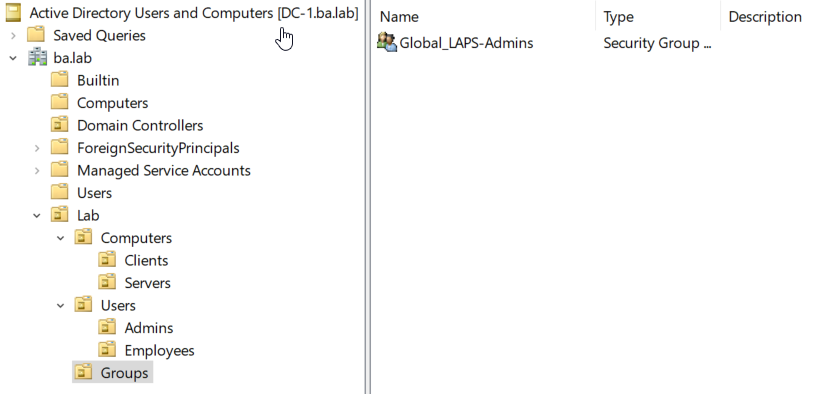
\includegraphics[width=0.7\linewidth]{../img/LAPS/Laps-Admins.png}
    \caption{LAPS Active Directory Gruppe}
\end{figure}

Nach dem erstellen der Gruppe, muss zusätzlich noch eine Berechtigung auf der OU für die Gruppe eingerichtet werden.
Dazu muss ASEdit und die Eigenschaften der OU geöffnet werden. Im ``Security'' Tab
\begin{figure}[H]
    \centering
    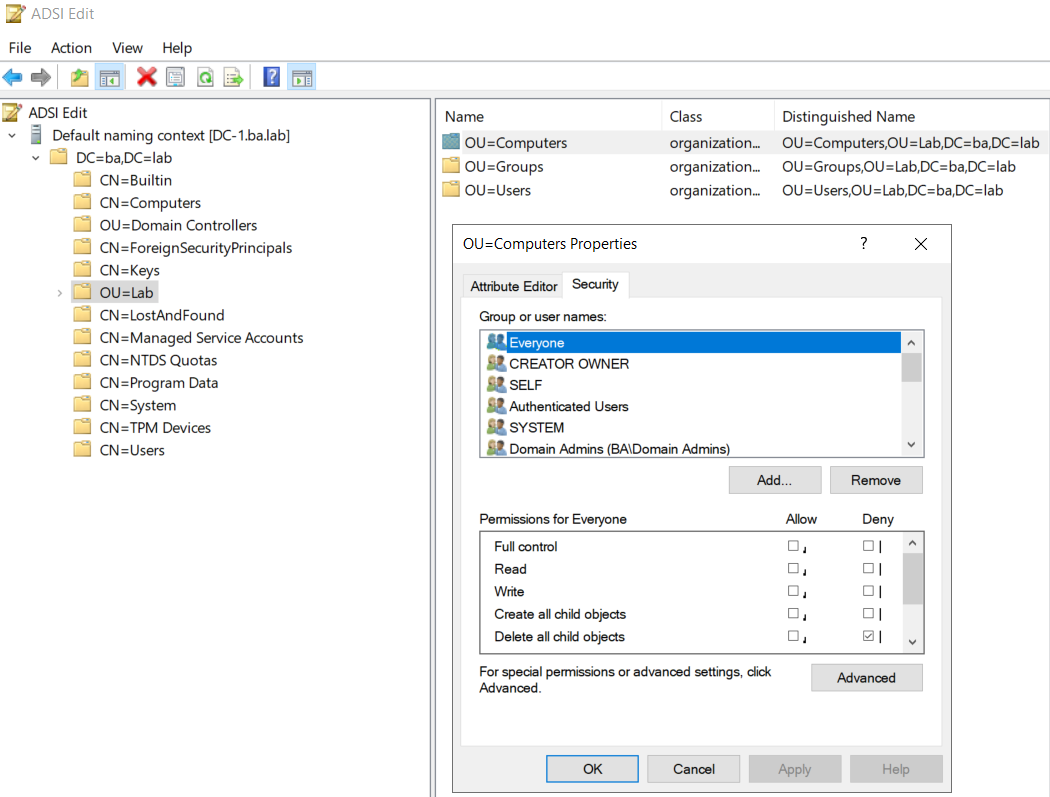
\includegraphics[width=0.7\linewidth]{../img/LAPS/ASEdit.png}
    \caption{ASEdit}
\end{figure}

%TODO: Add Picture 

Unter ``Advanced'' muss die neue Gruppe hinzugefügt werden mit der Berechtigung ``All Extended Rights''.
Nun muss für LAPS noch die Verknüpfung zwischen dieser Gruppe und der OU erstellt werden.
Dies kann mit Powershell erledigt werden:
\begin{lstlisting}
Set-AdmPwdReadPasswordPermission -OrgUnit "Computers" -AllowedPrincipals Global_LAPS-Admins
Set-AdmPwdResetPasswordPermission -OrgUnit "Computers" -AllowedPrincipals Global_LAPS-Admins
\end{lstlisting}
Die Read Berechtigung erlaubt das Lesen der Passwörter.
Die Reset Berechtigung erlaubt das setzten eines Ablaufdatums eines Passwortes.
Die Berechtigung kann nun noch mti Powershell überprüft werden:
\begin{lstlisting}
Find-AdmPwdExtendedrights -identity "Computers"
\end{lstlisting}


\subsection{LAPS aktivieren}
Zum Schluss muss LAPS noch mit einer neuen Group Policy aktiviert werden.

Im Group Policy Management muss eine neue Group Policy erstellt werden, welche mit der gleichen OU verknüpft ist, wie die Group Policy für das Deployment.
\begin{figure}[H]
    \centering
    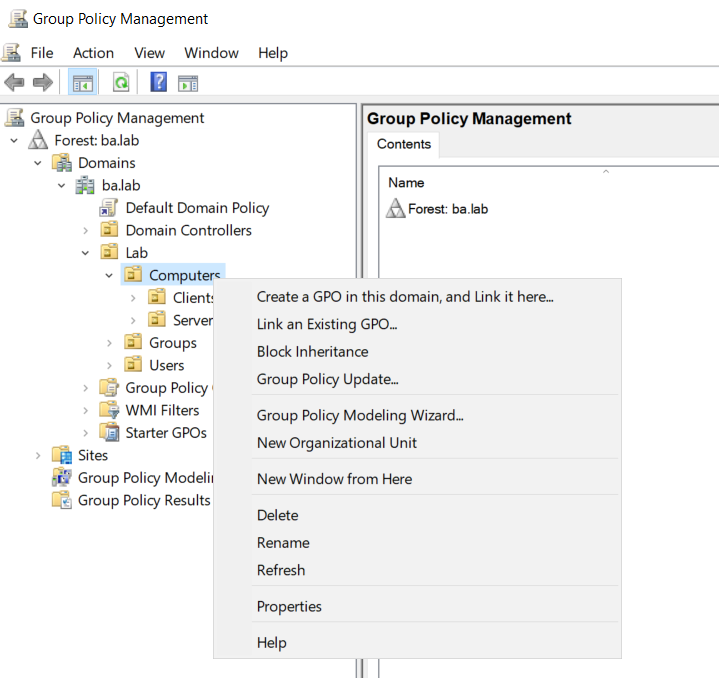
\includegraphics[width=0.7\linewidth]{../img/LAPS/GPO-Create-New.png}
    \caption{Neue GPO für LAPS Deployment}
\end{figure}
%2. Edit Policy and go to Computer Configuration > Policies > Administrative Templates > Laps [enable-laps]
%
%3. Enable Password Settings and define how: best 14 characters and change all
%
%
%